\documentclass[12pt, a4paper]{article}

\usepackage[hmargin=2.5cm, vmargin=2cm]{geometry}
\usepackage{amsthm, amssymb, mathtools, yhmath, graphicx}
\usepackage{fontspec, type1cm, titlesec, titling, fancyhdr, tabularx}
\usepackage{color}
\usepackage{unicode-math}
\usepackage{float}
\usepackage{subfig}
\usepackage{hhline}
\usepackage{comment}
\usepackage{siunitx}
\usepackage{csvsimple}
\usepackage{subcaption}

\usepackage[CheckSingle, CJKmath]{xeCJK}
\usepackage{CJKulem}
\usepackage{enumitem}
\usepackage{tikz}
\usepackage[siunitx]{circuitikz}
\usepackage{wrapfig}
%\setCJKmainfont[BoldFont=cwTex Q Hei]{cwTex Q Ming}
%\setCJKsansfont[BoldFont=cwTex Q Hei]{cwTex Q Ming}
%\setCJKmonofont[BoldFont=cwTex Q Hei]{cwTex Q Ming}
\setCJKmainfont[BoldFont=cwTeX Q Hei]{cwTeX Q Ming}

\def\normalsize{\fontsize{12}{18}\selectfont}
\def\large{\fontsize{14}{21}\selectfont}
\def\Large{\fontsize{16}{24}\selectfont}
\def\LARGE{\fontsize{18}{27}\selectfont}
\def\huge{\fontsize{20}{30}\selectfont}

%\titleformat{\section}{\bf\Large}{\arabic{section}}{24pt}{}
%\titleformat{\subsection}{\large}{\arabic{subsection}.}{12pt}{}
%\titlespacing*{\subsection}{0pt}{0pt}{1.5ex}

\parindent=24pt

\DeclarePairedDelimiter{\abs}{\lvert}{\rvert}
\DeclarePairedDelimiter{\norm}{\lVert}{\rVert}
\DeclarePairedDelimiter{\inpd}{\langle}{\rangle}
\DeclarePairedDelimiter{\ceil}{\lceil}{\rceil}
\DeclarePairedDelimiter{\floor}{\lfloor}{\rfloor}

\newcommand{\unit}[1]{\:(\text{#1})}
\newcommand{\df}[1]{\mathop{}\!\mathrm{d^#1}}
\newcommand{\img}{\mathrm{i}}
\newcommand{\dD}{\mathrm{d}}
\newcommand{\dI}{\,\mathrm{d}}

\title{ \bf {\Huge 電子電路實驗3:CMOS Operational Amplifier}\\ 實驗結報}
\author{B02901178 江誠敏}

\begin{document}

\maketitle


\section{實驗結果}
\subsection{DC Analysis}

\begin{minipage}[t]{0.5\textwidth}
\begin{tabular}{p{3cm}p{3cm}}
	\hline
  Item & Voltage\\
	\hhline{==}
  $V_{GD5}$ & $\SI{2.2}\V$ \\
  $V_{GD7}$ & $\SI{2.2}\V$ \\
  $V_{GD8}$ & $\SI{0.0}\V$ \\
  $V_{GD1}$ & $\SI{5.6}\V$ \\
  $V_{GD2}$ & $\SI{3.6}\V$ \\
  $V_{GD3}$ & $\SI{0.0}\V$ \\
  $V_{GD4}$ & $\SI{1.8}\V$ \\
	\hline
\end{tabular}
\end{minipage}%
\begin{minipage}[t]{0.5\textwidth}
\begin{tabular}{p{3cm}p{3cm}}
	\hline
  Item & Voltage\\
	\hhline{==}
  $V_{A}$ & $\SI{-0.09}\V$ \\
  $V_{E}$ & $\SI{-5.0}\V$ \\
  $V_{F}$ & $\SI{-0.07}\V$ \\
	\hline
\end{tabular}
\end{minipage}
\subsection{DC Sweep}
\vspace*{-0.5cm}
\begin{figure}[H]
\begin{center}
  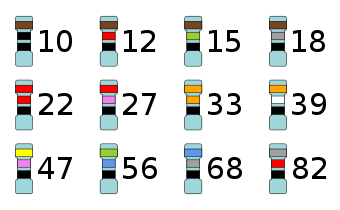
\includegraphics[width=0.75\textwidth]{fig1.pdf}
\end{center}
\label{fig:}
\end{figure}

\subsection{AC Analysis}

\begin{center}
  \begin{tabular}{p{4cm}p{4cm}}
	\hline
  Item & Voltage\\
	\hhline{==}
  $A_{M, 1}$ & $550.0$ \\
  $V_F$ & $\SI{360}\mV$ \\
  Distortion $V_i$ & $\SI{20}\V_{p-p}$ \\
	\hline
\end{tabular}
\end{center}

\subsection{AC Sweep}
\vspace*{-0.5cm}
\begin{figure}[H]
\begin{center}
  \includegraphics[width=0.75\textwidth]{fig2.pdf}
\end{center}
\caption{Bode plot}
\label{fig:}
\end{figure}

\section{心得}
這次的實驗超級花時間的,每個人都做的一把鼻涕一把眼淚,
本來10點左右就會陸陸續續開始有人做完實驗了,這次好像到了
11點都還沒有人做完,
更慘的是還聽說期末考有很大的機率就是考這個實驗。不過好
消息是從這次實驗開始結報都不用寫問題討論了!助教人真是
太好了!
\end{document}

